%%%%%%%%%%%%%%%%%%%%%%%%%%%%%%%%%%%%%%%%%%%%%%%
%Consuntivo a finire
%Version: 0.0.1
%Author: Nicolò Bissacco(nickbissa@gmail.com)
%Creation Date: 2013-12-19
%Change Table
%Relase		Author			Date		Object of the changed
%%%%%%%%%%%%%%%%%%%%%%%%%%%%%%%%%%%%%%%%%%%%%%%%
\pagebreak
\section{Consuntivo corrente}
\label{Consuntivo}
In questa sezione viene presentato il bilancio tra il preventivo e il consuntivo.
Tale bilancio può essere:
\begin{itemize}
	\item \textbf{Positivo:} il preventivo ha superato il consuntivo;
	\item \textbf{Negativo:} il consuntivo ha superato il preventivo;
	\item \textbf{In pari:} il consuntivo coincide con il preventivo.
\end{itemize}
%%%%%%%%%%%%%%%%%%%%%%%%%%%%%%%%%%%%%%
%									%
%       CONSUNTIVO ANALISI              %
%									%
%%%%%%%%%%%%%%%%%%%%%%%%%%%%%%%%%%%%%%
\subsection{Fase A}
\label{ConsuntivoAnalisi}
	Si riporta di seguito il consuntivo riguardante la fase A (FA).
	\\ La seguente tabella illustra le ore pianificate e tra parentesi la differenza tra il preventivo e il consuntivo suddiviso per ruoli; viene inoltre riportato il costo preventivato e la differenza di costo tra parentesi. Vengono poi rappresentati i totali del preventivo e del consuntivo, specificando inoltre la differenza oraria ed economica tra preventivo e consuntivo. Il segno positivo riguardante i costi indica che il consuntivo ha superato il preventivo e quindi il bilancio è negativo.
	
	\begin{table}[!h]
		\centering
		\begin{tabular}{|l|c|c|}
			\hline
			Ruolo & Ora & Costo\\
			\hline
			Amministratore & 20 (-1) & 400 (-20)\\
			Responsabile & 18 (+1) & 540 (+30)\\
			Analista & 65 (-1) & 1.625 (-25)\\
			Verificatore & 41 (+1) & 902 (+22)\\
			Progettista & 0 & 0\\
			Programmatore & 0 & 0\\	
			\hline
			preventivo & 144 & 3.467\\
			consuntivo & 144 & 3.474\\
			differenza & 0 & +7\\
			\hline			
		\end{tabular}
		\caption{Consuntivo per Ruolo, FA}
	\end{table}
		Il seguente grafico illustra la differenza tra le ore pianificate e le ore realmente impiegate suddivise per ruolo per la fase A.
\begin{figure}[!h]
	\centering
	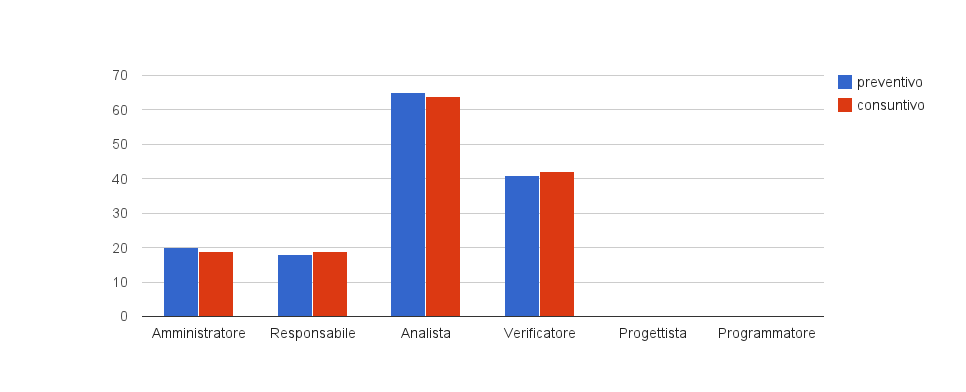
\includegraphics[width=1\textwidth] {./content/Immagini/consA}
	\caption{Bilancio per ruolo, FA}
	\label{bilA}
\end{figure}	 
	\\La seguente tabella, invece, riporta le ore pianificate per ogni risorsa suddivise per ruoli rivestiti e tra parantesi la differenza di ore tra consuntivo e preventivo.	
	\begin{table} [!h]
		\tableResource
		Adami Alberto &10 (0) & & 7 (0) & 3 (0) & & & 20 (0)\\
		Bissacco Nicolò &10 (-1) & 4 (0) & 7 (0) & & & &21 (-1)\\
		Feltre Beatrice & & 8 (+1) & 12 (-2) & & & & 20 (-1)\\
		Luisetto Luca & & & 13 (+1) & 8 (0) & & & 21 (+1)\\
		Magnabosco Nicola & & 6 (0) & &15 (+1) & & & 21(+1)\\
		Martignago Jimmy & & & 15 (0) & 6 (0) & & & 21 (0)\\
		Scapin Davide & & & 11 (0) & 9 (0) & & & 20 (0)\\ \hline
		\end{tabular} \caption{Consuntivo per Risorsa, FA}
		\end{center}
	\end{table}
	\pagebreak
	\subsubsection{Preventivo a finire}
	La seguente tabella illustra il consuntivo corrente, dall'inizio dei lavori fino ad oggi.
	\begin{table}[!h]
		\centering
		\begin{tabular}{|l|c|c|}
			\hline
			Ruolo & Ora & Costo\\
			\hline
			Amministratore & 19 & 380\\
			Responsabile & 19 & 570\\
			Analista & 64 & 1.600\\
			Verificatore & 42 & 924\\
			Progettista &  & \\
			Programmatore & & \\	
			\hline
			Totale &144 &3.474\\
			\hline			
		\end{tabular}
		\caption{Consuntivo corrente fino  alla RR}
	\end{table}
	
	\subsubsection{Conclusioni}
	\label{CCA}
	Svolgendo le attività pianificate e riportate nel diagramma di Gantt\glossario{}, in figura \ref{DiagrammaAnalisiGantt}, è stato necessario gestire differentemente la distribuzione oraria dei vari ruoli.\\
	Il gruppo ha comunque impiegato lo stesso numero di ore per completare la fase A provocando una piccola variazione di costo nel bilancio, infatti attualmente il \textbf{bilancio} risulta essere \textbf{negativo}. Tale passivo non andrà ad influenzare il costo totale del progetto preventivato in quanto le ore impiegate in questa fase non sono state conteggiate nel calcolo del preventivo e quindi non imputabili al Proponente.
\pagebreak
%%%%%%%%%%%%%%%%%%%%%%%%%%%%%%%%%%%%%%
%									%
%  CONSUNTIVO ANALISI INCREMENTALE	%
%									%
%%%%%%%%%%%%%%%%%%%%%%%%%%%%%%%%%%%%%%
\subsection{Fase B}
\label{consuntivoAnalisiIncr}
	Si riporta di seguito il consuntivo riguardante la fase B (FB).
	\\ La seguente tabella illustra le ore pianificate e tra parentesi la differenza tra il preventivo e il consuntivo suddiviso per ruoli; viene inoltre riportato il costo preventivato e la differenza di costo tra parentesi. Vengono poi rappresentati i totali del preventivo e del consuntivo, specificando inoltre la differenza oraria ed economica tra consuntivo e preventivo.
	\begin{table}[!h]
		\centering
		\begin{tabular}{|l|c|c|}
			\hline
			Ruolo & Ora & Costo\\
			\hline
			Amministratore & 7 (0) & 140 (0)\\
			Responsabile & 3 (0) & 90 (0)\\
			Analista & 27 (-2) & 675 (-50)\\
			Verificatore & 22 (-1) & 484 (-22)\\
			Progettista & 0 & 0\\
			Programmatore & 0 & 0\\	
			\hline
			preventivo & 59 & 1.389\\
			consuntivo & 56& 1.317 \\
			differenze & -3& -72 \\
			\hline			
		\end{tabular}
		\caption{Consuntivo per Ruolo, FB}
	\end{table}
		\\Il seguente grafico illustra la differenza tra le ore pianificate e le ore realmente impiegate suddivise per ruolo per la fase B.
\begin{figure}[h]
	\centering
	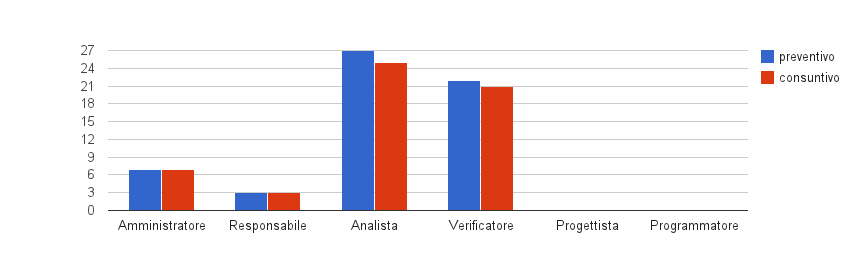
\includegraphics[width=1.1\textwidth] {./content/Immagini/consAI.png}
	\caption{Bilancio per ruolo, FB}
	\label{bilAI}
\end{figure}	 
		\\La seguente tabella, invece, riporta le ore pianificate per ogni risorsa suddivise per ruoli rivestiti e tra parantesi la differenza di ore tra consuntivo e preventivo.	
	\begin{table} [!h]
		\tableResource
		Adami Alberto & & &  & 8 (0) & & & 8 (0)\\
		Bissacco Nicolò & & & 7 (0) & & & & 7 (0)\\
		Feltre Beatrice & & & & 8 (0) & & & 8 (0)\\
		Luisetto Luca & & 3 (0)& & 6 (-1) & & & 9 (-1)\\
		Magnabosco Nicola & & & 9 (-2) & & & & 9 (-2)\\
		Martignago Jimmy & & & 8 (0) & 6 (0)& & & 8 (0)\\
		Scapin Davide & 7 (0) & & 3 (0) & & & & 10 (0)\\
		\hline
		\end{tabular} 
		\caption{Consuntivo per Risorsa, FB}
		\end{center}
	\end{table}
	\pagebreak
	
	\subsubsection{Preventivo a finire}
	La seguente tabella illustra il consuntivo corrente, dall'inizio dei lavori fino ad oggi. Si considerano solo le ore e i costi imputabili al proponente.
	\begin{table}[!h]
		\centering
		\begin{tabular}{|l|c|c|}
			\hline
			Ruolo & Ora & Costo\\
			\hline
			Amministratore & 7 & 140\\
			Responsabile & 3 & 90\\
			Analista & 25 & 625\\
			Verificatore & 21 & 462\\
			Progettista &  & \\
			Programmatore & & \\	
			\hline
			Totale &56 &1.317\\
			Risparmio& & 72\\
			\hline			
		\end{tabular}
		\caption{Consuntivo corrente dopo fase B}
	\end{table}
	\subsubsection{Conclusioni}
	\label{CCAI}
	Svolgendo le attività pianificate e riportate nel diagramma di Gantt\glossario{}, in figura \ref{DiagrammaIncrementale}, si sono utilizzate meno ore di quelle previste, portando ad un risparmio di \EUR{72} che potrà poi essere investito per le attività nella fase C (FC) principalmente a sostegno dell'attività di verifica. 
	Il bilancio per la fase B (FB) risulta essere \textbf{positivo}.
	\pagebreak
%%%%%%%%%%%%%%%%%%%%%%%%%%%%%%%%%%%%%%%%%%%%%%
%											%
%  CONSUNTIVO PROGETTAZIONE ARCHITETTURALE	%
%											%
%%%%%%%%%%%%%%%%%%%%%%%%%%%%%%%%%%%%%%%%%%%%%%
\subsection{Fase C}
\label{consuntivoPrArchi}
	Si riporta di seguito il consuntivo riguardante la fase C (FC).
	\\ La seguente tabella illustra le ore pianificate e tra parentesi la differenza tra il preventivo e il consuntivo suddiviso per ruoli; viene inoltre riportato il costo preventivato e la differenza di costo tra parentesi. Vengono poi rappresentati i totali del preventivo e del consuntivo, specificando inoltre la differenza oraria ed economica tra preventivo e consuntivo.
	\begin{table}[!h]
		\centering
		\begin{tabular}{|l|c|c|}
			\hline
			Ruolo & Ora & Costo\\
			\hline
			Amministratore & 8 (0) & 160 (0)\\
			Responsabile & 11 (0) & 330 (0)\\
			Analista & 19 (-3) & 475 (-75)\\
			Verificatore & 46 (+3) & 1.012 (+66)\\
			Progettista & 99 (+2) & 1.485 (+30)\\
			Programmatore & 0 & 0\\	
			\hline
			preventivo & 183 & 3.462\\
			consuntivo & 185 & 3.483\\
			differenze & +2 & +21 \\
			\hline			
		\end{tabular}
		\caption{Consuntivo per Ruolo, FC}
	\end{table}
	\\Il seguente grafico illustra la differenza tra le ore pianificate e le ore realmente impiegate suddivise per ruolo per la fase C.
\begin{figure}[h]
	\centering
	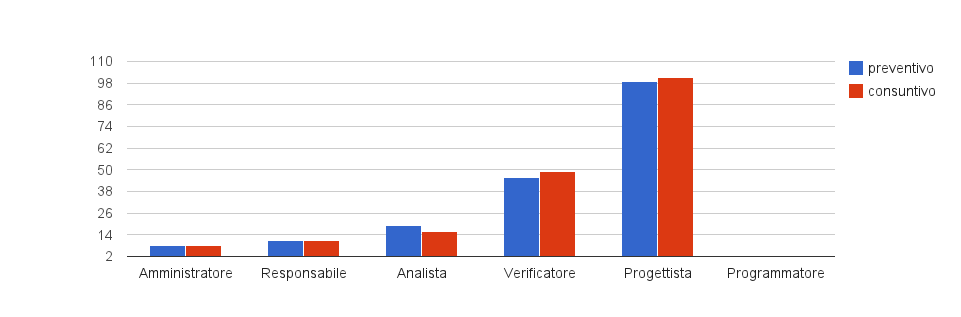
\includegraphics[width=1.1\textwidth] {./content/Immagini/consPA.png}
	\caption{Bilancio per ruolo, FC}
	\label{bilPA}
\end{figure}	 
		\\La seguente tabella, invece, riporta le ore pianificate per ogni risorsa suddivise per ruoli rivestiti e tra parantesi la differenza di ore tra consuntivo e preventivo.	
	\begin{table} [!h]
		\tableResource
		Adami Alberto 	  & & 5 (0) & 10 (-2) & & 9 (+3) & & 24 (+1)\\
		Bissacco Nicolò   & & & & 20 (-1) & 6 (+2) & & 26 (+1)\\
		Feltre Beatrice   & 4 (0) & & & & 22 (+1) & & 26 (+1)\\
		Luisetto Luca 	  & 4 (0)& & & & 23 (0)& & 27 (0)\\
		Magnabosco Nicola & & 4 (0)& 9 (-1) & & 14 (+2) & & 27 (+1)\\
		Martignago Jimmy  & & 2 (0)& & 18 (+3) & 6 (-6) & & 26 (-3)\\
		Scapin Davide 	  & & & & 8 (+1) & 19 (0)& & 27 (+1)\\ \hline
		\end{tabular} \caption{Consuntivo per Risorsa, FC}
		\end{center}
	\end{table}
	\pagebreak
	\subsubsection{Preventivo a finire}
	La seguente tabella illustra il consuntivo corrente, dall'inizio dei lavori fino ad oggi. Si considerano solo le ore e i costi imputabili al proponente.
	\begin{table}[!h]
		\centering
		\begin{tabular}{|l|c|c|}
			\hline
			Ruolo & Ora & Costo\\
			\hline
			Amministratore & 15& 300\\
			Responsabile & 14 & 420\\
			Analista & 41 & 1.025\\
			Verificatore & 70 & 1.540\\
			Progettista & 101 &1.515 \\
			Programmatore & & \\	
			\hline
			Totale &241 &4.800\\
			Risparmio& & 51\\
			\hline			
		\end{tabular}
		\caption{Consuntivo corrente dopo RP}
	\end{table}
	
	\subsubsection{Conclusioni}
	\label{CCPA}
Svolgendo le attività pianificate e riportate nel diagramma di Gantt\glossario{}, in figura \ref{DiagrammaArchitetturale}, sono state necessarie alcune ore in più per poterle portare a termine e una ripartizione diversa tra i ruoli.\\
Potendo contare economicamente su quanto risparmiato nella fase B (FB) che ammontava a \EUR{72}, l'aumento del costo per la fase C (FC), è stato largamente ricoperto, disponendo ancora di una piccola somma (che ammonta a \EUR{51}) da poter investire nella fase successiva. \\
Il bilancio della sola fase C (FC), seppur di poco, si chiude in \textbf{negativo}, ma il bilancio complessivo rimane \textbf{positivo}.
\pagebreak
%%%%%%%%%%%%%%%%%%%%%%%%%%%%%%%%%%%%%%%%%%%%%%%%%%
%												%
%  CONSUNTIVO PROGETTAZIONE DETTAGLIO E CODIFICA	%
%												%
%%%%%%%%%%%%%%%%%%%%%%%%%%%%%%%%%%%%%%%%%%%%%%%%%%
\subsection{Fase D}
\label{consuntivoD}
	Si riporta di seguito il consuntivo riguardante la fase D (FD).
	\\ La seguente tabella illustra le ore pianificate e tra parentesi la differenza tra il preventivo e il consuntivo suddiviso per ruoli; viene inoltre riportato il costo preventivato e la differenza di costo tra parentesi. Vengono poi rappresentati i totali del preventivo e del consuntivo, specificando inoltre la differenza oraria ed economica tra preventivo e consuntivo.
	\begin{table}[!h]
		\centering
		\begin{tabular}{|l|c|c|}
			\hline
			Ruolo & Ora & Costo\\
			\hline
			Amministratore & 9 (-3) & 180 (-60)\\
			Responsabile & 11 (-4) & 330 (-120)\\
			Analista & 3 (-2) & 75 (-50)\\
			Verificatore & 111 (+6) & 2.442 (+132)\\
			Progettista & 105 (+8) & 1.575 (+120)\\
			Programmatore & 180 (0) & 1.770 (0)\\	
			\hline
			preventivo & 357 & 6.372\\
			consuntivo & 362 & 6.394\\
			differenze & +5 & +22 \\
			\hline			
		\end{tabular}
		\caption{Consuntivo per Ruolo, FD}
	\end{table}
	\\Il seguente grafico illustra la differenza tra le ore pianificate e le ore realmente impiegate suddivise per ruolo per la fase D.
\begin{figure}[h]
	\centering
	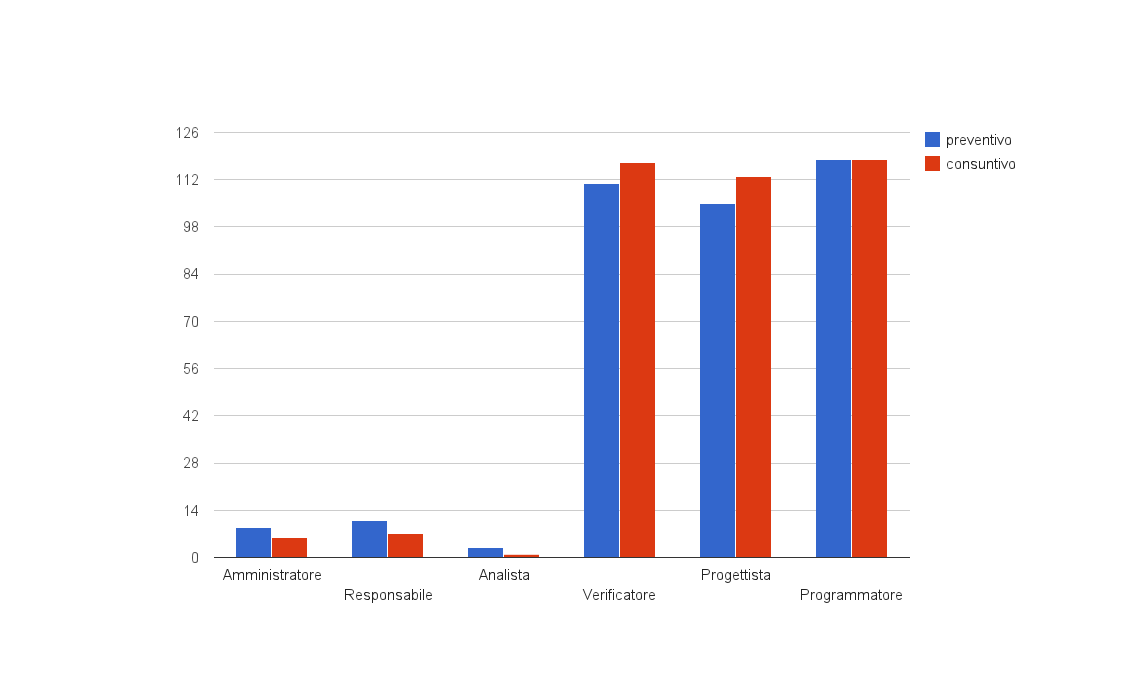
\includegraphics[width=1\textwidth] {./content/Immagini/consD.png}
	\caption{Bilancio per ruolo, FD}
	\label{bilD}
\end{figure}	 
		\\La seguente tabella, invece, riporta le ore pianificate per ogni risorsa suddivise per ruoli rivestiti e tra parantesi la differenza di ore tra consuntivo e preventivo.	
	\begin{table} [!h]
		\tableResource
		Adami Alberto 	  &  &  & &28 (+2) & 23 (0) & & 51 (+2)\\
		Bissacco Nicolò   &  &  & & 17 (0) & 25 (0) & 10(0)& 52 (0)\\
		Feltre Beatrice   &  &  & & 30 (0) & 22 (0) & & 52 (0)\\
		Luisetto Luca 	  &  &  & &25 (0) & & 26 (0) & 51 (0)\\
		Magnabosco Nicola &9 (-3)& & & & 4 (+3) & 40 (0)& 53 (0)\\
		Martignago Jimmy  &  & &3 (-2) & & 31 (+5) &14 (0)& 48 (+3)\\
		Scapin Davide 	  & &11 (-4)& & 11 (+4) & & 28 (0)& 50 (0)\\ \hline
		\end{tabular} \caption{Consuntivo per Risorsa, FD}
		\end{center}
	\end{table}
	\pagebreak
	\subsubsection{Preventivo a finire}
	La seguente tabella illustra il consuntivo corrente, dall'inizio dei lavori fino ad oggi. Si considerano solo le ore e i costi imputabili al proponente.
	\begin{table}[!h]
		\centering
		\begin{tabular}{|l|c|c|}
			\hline
			Ruolo & Ora & Costo\\
			\hline
			Amministratore & 21& 420\\
			Responsabile & 21 & 630\\
			Analista & 42 & 1.050\\
			Verificatore & 187 & 4.114\\
			Progettista & 214 &3.210 \\
			Programmatore &118 & 1.770\\	
			\hline
			Totale &603&4.800\\
			Risparmio& & 29\\
			\hline			
		\end{tabular}
		\caption{Consuntivo corrente dopo RQ}
	\end{table}
	\subsubsection{Conclusioni}
	\label{CCD}
Svolgendo le attività pianificate e riportate nel diagramma di Gantt\glossario{}, in figura \ref{DiagrammaCodifica}, sono state necessarie alcune ore in più per poterle portare a termine e una ripartizione diversa tra i ruoli. In particolare le ore preventivate per l'analista sono state ridotte in quanto gli esiti della revisione di progettazione, sono stati positivi a meno di qualche postilla facilmente rimediabile. Si è inoltre dovuto investire maggiormente nel ruolo del progettista per poter risistemare in modo adeguato l'architettura del sistema precedentemente progettata. Sono state aumentate le ore per la verifica dei documenti. Le ore riguardanti i programmatori invece sono state sufficienti.\\
Potendo contare economicamente su quanto risparmiato nella fase C (FC) che ammontava a \EUR{51}, l'aumento del costo per la fase  D (FD), è stato largamente ricoperto, disponendo ancora di una piccola somma (che ammonta a \EUR{29}) da poter investire nella fase successiva. \\
Il bilancio della sola fase D (FD), seppur di poco, si chiude in \textbf{negativo}, ma il bilancio complessivo rimane \textbf{positivo}.\\
La somma risparmiata in questa fase, verrà investita nella fase successiva soprattutto per le attività di verifica e validazione del prodotto.
\pagebreak
%%%%%%%%%%%%%%%%%%%%%%%%%%%%%%%%%%%%%%
%									%
%  CONSUNTIVO VERIFICA E VALIDAZIONE	%
%									%
%%%%%%%%%%%%%%%%%%%%%%%%%%%%%%%%%%%%%%
\subsection{Fase E}
\label{consuntivoE}
	Si riporta di seguito il consuntivo riguardante la fase E (FE).
	\\ La seguente tabella illustra le ore pianificate e tra parentesi la differenza tra il preventivo e il consuntivo suddiviso per ruoli; viene inoltre riportato il costo preventivato e la differenza di costo tra parentesi. Vengono poi rappresentati i totali del preventivo e del consuntivo, specificando inoltre la differenza oraria ed economica tra preventivo e consuntivo.
	\begin{table}[!h]
		\centering
		\begin{tabular}{|l|c|c|}
			\hline
			Ruolo & Ore & Costo\\
			\hline
			Amministratore & 9 (-7) & 180 (-140)\\
			Responsabile & 9 (-8) & 210 (-180)\\
			Analista &  & \\
			Verificatore & 61 (-11) & 1.342 (-242)\\
			Progettista & 105 (+8) & 1.575 (+75)\\
			Programmatore & 14 (+33) & 210 (+495)\\	
			\hline
			preventivo & 111 & 2.242\\
			consuntivo & 125 & 2.250\\
			differenze & +14 & +8 \\
			\hline			
		\end{tabular}
		\caption{Consuntivo per Ruolo, FE}
	\end{table}
	\\Il seguente grafico illustra la differenza tra le ore pianificate e le ore realmente impiegate suddivise per ruolo per la fase E. \\ \\ \\
\begin{figure}[!h]
	\centering
	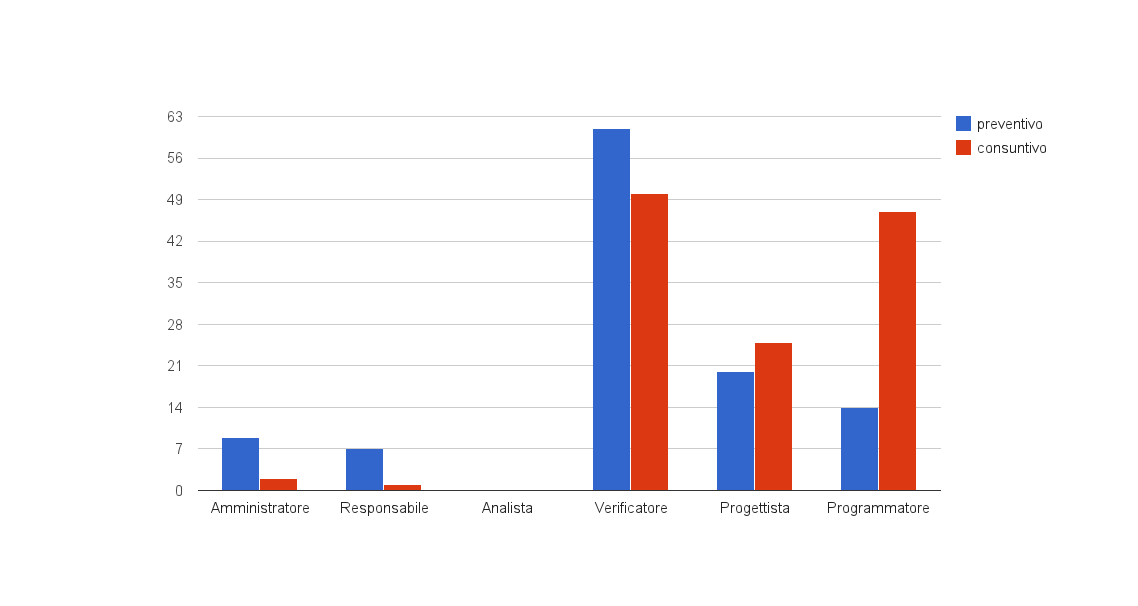
\includegraphics[width=1.2\textwidth] {./content/Immagini/consE.png}
	\caption{Bilancio per ruolo, FE}
	\label{bilE}
\end{figure}	 
		\\ \\ \\
		La seguente tabella, invece, riporta le ore pianificate per ogni risorsa suddivise per ruoli rivestiti e tra parantesi la differenza di ore tra consuntivo e preventivo.\\
	\begin{table} [!h]
		\tableResource
		Adami Alberto 	   &  &  & &10(0)& & 7 (+1)&17 (+1)\\
		Bissacco Nicolò    &  &  & &15 (-6) & &0 (+9)&15 (+3)\\
		Feltre Beatrice    &7 (-7) & & &2 (+8)&0 (+3) &7 (-3) &16 (+1)\\
		Luisetto Luca 	   &  & 7 (-6)& &8 (0)& 0 (+9)& &15 (+3)\\
		Magnabosco Nicola  &  &  & &9 (-3)&5 (-2)&0 (+7) &14 (+2)\\
		Martignago Jimmy   &2 (0)&  & &17 (-8)&0 (+7) & 0 (+4)&19 (+3)\\
		Scapin Davide 	   &  & & & 8 (-2)&7 (-3) & 0 (+6) &15 (+1)\\ \hline
		\end{tabular} \caption{Consuntivo per Risorsa, FE}
		\end{center}
	\end{table}
	\\
	La seguente tabella illustra il consuntivo corrente, dall'inizio dei lavori fino ad oggi. Si considerano solo le ore e i costi imputabili al proponente.
	\begin{table}[!h]
		\centering
		\begin{tabular}{|l|c|c|}
			\hline
			Ruolo & Ora & Costo\\
			\hline
			Amministratore & 23& 460\\
			Responsabile & 22 & 660\\
			Analista & 42 & 1.050\\
			Verificatore & 237 & 5.214\\
			Progettista & 239 &3.585 \\
			Programmatore &165 & 2.475\\	
			\hline
			Totale &728&13.444\\
			Risparmio& & 21\\
			\hline			
		\end{tabular}
		\caption{Consuntivo corrente, ingresso in RA}
	\end{table}
	\subsubsection{Conclusioni}
	\label{CCE}
Svolgendo le attività pianificate e riportate nel diagramma di Gantt\glossario{}, in figura \ref{DiagrammaVerificaValidazione}, sono state necessarie alcune ore in più per poterle portare a termine e una ripartizione diversa tra i ruoli. In particolare le ore preventivate per il programmatore sono dovute aumentare a fronte dell'implementazione di componenti che hanno portato a dei problemi durante la codifica. Si sono potute ridurre i ruoli riguardanti l'amministratore e il responsabile in quanto non si sono riscontrate necessità di avere questi ruoli nella quantità preventivata a inizio lavori. Inoltre il progettista ha avuto un aumento di poche ore a seguito della revisione di qualifica e degli errori riguardanti l'architettura.\\
Potendo contare economicamente su quanto risparmiato nella fase D (FD) che ammontava a \EUR{29}, l'aumento del costo per la fase  E (FE), seppur di entità molto bassa (\EUR{8}) è stato ricoperto.
Il bilancio della sola fase E (FE), seppur di poco, si chiude in \textbf{negativo}, ma il bilancio complessivo rimane \textbf{positivo}.\\
\pagebreak